\section{Application Overview}
This thesis consists of two parts. The first of which is the~CAPI backend. It stores and retrieves data from and to the database via calls to the KAPI. It itself is called from the~mobile client app, called KenticoApp, through which the~user is able to communicate with the~system and manage his site.

The CAPI partially follows the representational state transfer (REST) architecture by using appropriate hyper text transfer protocols (Http). For example we use POST requests for creating or GET requests for reading resources from the backend. The usage of status codes, such as 200 for OK, 403 for forbidden or 503 for service unavailable, is also a RESTful convention. Our backend is stateless. This is achieved by using ATs instead of storing the user session across multiple Http requests. One of the reasons why we cannot call this application RESTful is it does not follow the fundamental concept of identifying all resources and relationships between them. For example our \textit{System} "resource" contains the method \textit{ClearCache()} and \textit{ShowEventlog()}. These should be identified in separate resources \textit{CacheClearer} and \textit{Eventlog}.

The communication between the CAPI and KenticoApp is ensured by Ajax using the JSON format. It is an effective way to broadcast information via a simple string.

\begin{figure}[ht!]
  \centering
  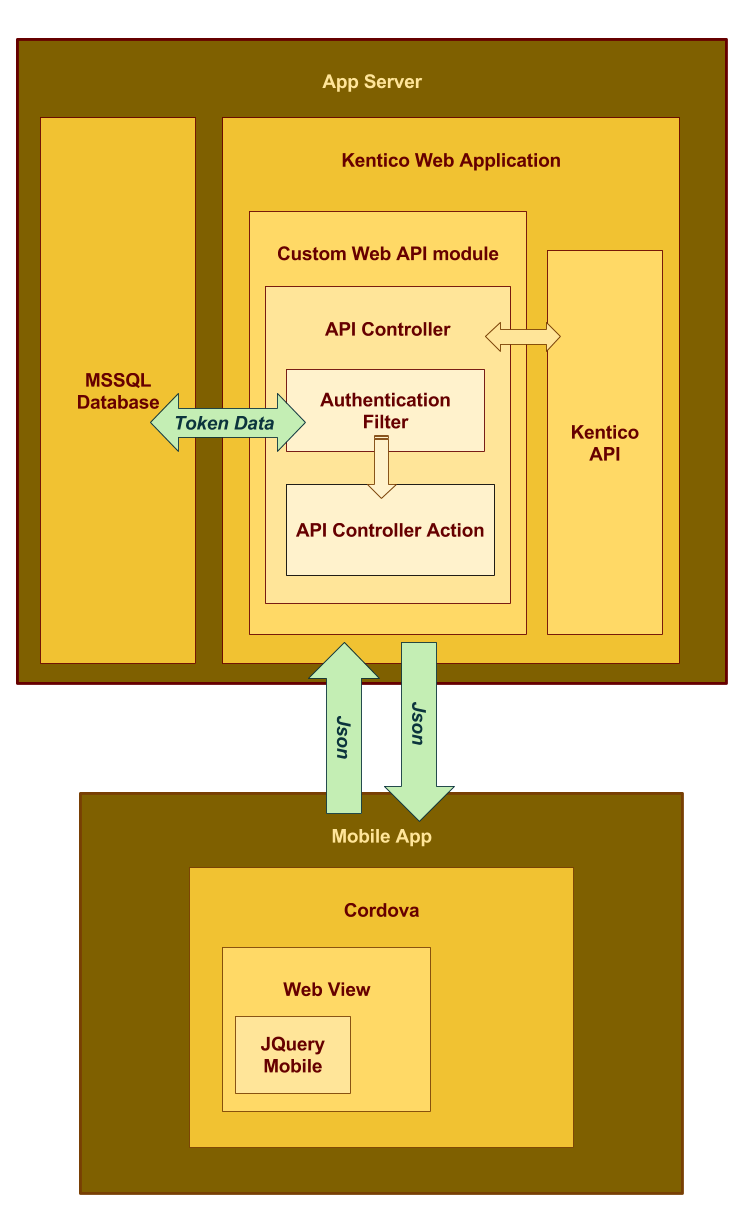
\includegraphics[width=\textwidth]{Images/Architecture.png}
  \caption{Architecture overview}
  \label{architectureOverview}
\end{figure}

\section{Extending Kentico} \label{implExtendingKentico}
\subsection{Custom Kentico Module}
The CAPI was created using the .Net framework. It uses KAPI calls and is called by the KenticoApp. For executing an API call, the user has to be signed into the system and have the proper authorization. 
TODO: 

\subsection{Kentico 9.0 API}

\section{Web API Application}
\subsection{Microsoft Web API 1.0}
TODO:API Controller, Filters, Recieving and sending response (JSON), REST: HttpError Codes, stateless, token, not restful
The API call structure is demonstrated in the illustrated code below. 
\lstset{style=sharpc, numbers=left}
\begin{lstlisting}
[Authorize]
[HttpPost]
[Route("kenticoapi/users/edit-user")]
public HttpResponseMessage EditUser([FromBody]JObject postData)
{
  string username, firstName, surname;
  try
  {
    username = postData["username"].ToObject<string>();
    firstName = postData["firstName"].ToObject<string>(); 
    surname = postData["surname"].ToObject<string>();
  }
  catch (Exception e)
  {
    return Request.CreateResponse(HttpStatusCode.ServiceUnavailable, new { errorMessage = e.Message });
  }
  try
  {
    UserInfo updateUser = UserInfoProvider.GetUserInfo(username);
    if (updateUser != null)
    {
      updateUser.FirstName = firstName;
      updateUser.LastName = surname;
      UserInfoProvider.SetUserInfo(updateUser);
    return Request.CreateResponse(HttpStatusCode.OK, new { user = updateUser });
    }
  } catch(Exception e)
  {
    return Request.CreateResponse(HttpStatusCode.ServiceUnavailable, new { errorMessage = e.Message });
  }
  return Request.CreateResponse(HttpStatusCode.ServiceUnavailable, new { errorMessage = "User is null" });
}
\end{lstlisting}
The annotation from the 1st is noted either in front of a particular method, or in front of a whole controller so that all its methods are affected. It which was implemented as our custom AuthenticatorFilter and checks if the user is authenticated so the call can be executed. If successfully authorized, the user is stored into the request properties from where he can be retrieved with the following command:
\lstset{style=sharpc, numbers = none}
\begin{lstlisting}
	UserInfo user = (UserInfo) Request.Properties["LoggedUserInfo"]
\end{lstlisting}
as it is done in the method \textit{GetCurrentUser()}.
Line 2 ensures that only POST requests are handled by the method. POST requests send data from the client to the server as opposed to GET requests which demand data from the server. In this example the system stores updated user information from the KenticoApp into the database. The 3rd line represents the route where the call can be accessed through the client app. The 4th line is the head of the method. Its return type enables the client to receive a \textit{StatusCode} and a value, which is the content of the Http response message. The parameters are passed on from the client as one object in the JSON format. On the lines 6 to 12 the JSON object is parsed into separate parameters as \textit{strings}. This is done in a \textit{try-catch} block to handle possible exceptions and return the proper response message on the line 15. The \textit{CreateResponse()} method is of the class \textit{Request} and its parameters are the status code \textit{503 service unavailable} and an object with the error message of the caught exception from line 13. The line 19 gets the user with the parsed \textit{username} and stores it in the variable called \textit{updateUser} of the type \textit{UserInfo}. This type is defined in the KAPI documentation and has attributes such as \textit{username}, \textit{user ID}, \textit{user first} and \textit{last name}, etc. Line 20 checks if the \textit{updateUser} is not \textit{null}. Lines 22 and 23 change the \textit{updateUser}'s first and last name. On the line 24 the \textit{updateUser} is inserted in the database. Line 25 returns the status code \textit{200 OK} and the \textit{updateUser} object in JSON format. The lines 27 to 30 are similar to lines 13 to 16. If \textit{updateUser} is \textit{null} the response is status code \textit{503}, the same as on line 15, and the error message \textit{"User is null"}. 

\subsection{CAPI Token Management}
For user authentication we decided to use access tokens (AT). ATs are leveraged to secure the communication between a user and the system. After signing in the user is given a random generated unique AT by the system which stores it in its database. Before every API call, the system requires the user's AT and then checks it against the database. For the call to be executed the AT has to exist in the database with the corresponding user ID and must not be expired. If this is not the case the user is redirected to the welcome page, where he has to sign in. To represent and store the ATs in the database in our project we were inspired by the layered application design pattern, more specifically by its data access layer (DAL). This pattern is used to ensure security and scalability of an application by partitioning it into three layers. The first and lowest layer is needed to operate the database called DAL, it represents entities. The next layer is the business logic layer which contains the logic of the system and the last one is the presentation layer utilised to display the application through a UI to users. For the purpose of this thesis we decided to represent the ATs as an entity using the Entity Framework. The entity contains the user identification (ID), a unique pseudo-random code and an expiration date and time (expiration) as can be seen in the following example code. 
\lstset{style=sharpc, numbers=left}
\begin{lstlisting}
 public class Token
    {
        [Required]
        public int UserID { get; set; }
        [Required][Key]
        public string Code { get; set; }
        [Required]
        public DateTime Expiration { get; set; }
    }
\end{lstlisting}
The ID is of the type \textit{int} and is equal to the user's ID who "owns" the AT. The code is type \textit{string} and is generated with the pseudo-random number generator \textit{Random}. \textit{The chosen numbers are not completely random because a mathematical algorithm is used to select them, but they are sufficiently random for practical purposes.}\cite{msdn_documentation_system_random} Right after generating the code is tested against the database if no AT with the same one exists. If the code is already taken, another one is generated and tested. If not, the token entity is assigned the code, user ID and date and time 10 minutes from the assignment. The expiration is of the type \textit{DateTime}. After every executed API call the AT's expiration is set to 10 minutes from calling. 
Before every API call the system searches its database for expired ATs and deletes them. 

\section{Cordova Mobile Application}
\subsection{Apache Cordova}
For the~implementation of the~mobile app we leveraged the Apache Cordova framework (ACF). The~reason being it is less demanding to learn and supports seven platforms. As opposed to the~Xamarin framework (XF) supporting only three. Even though XF should be faster than ACF, and therefore offer a smoother user experience, the~difference between execution times of non performance sensitive apps on today's devices is negligible. We did not consider development in native languages, such as Android Java or iOS SWIFT, because of their steep learning curve and the ability to deploy only to one platform. The development was divided into two stages. For creating the UI  we decided to use JQuery Mobile. It is an~HTML5-based UI framework which allows users to design aesthetically pleasing mobile elements by utilising the~languages CSS and HTML. Document object model (DOM) elements are individual parts of a web page described by tags such as div, span, input or others. These tags assign styling and properties to elements. For the DOM manipulation we used the~JQuery library which has a~small learning curve and offers a~fast way to add, modify, style and delete elements or change their~behaviour. It also offers a set o handy helper functions which provide easy to use interface for frequently used operations in web development, e.g. \textit{Ajax()}.
TODO: Cordova vs. native vs. Xamarin, PhoneGap, Cordova wrapper
\subsection{JQuery Mobile}
Jquery Mobile is an~open source HTML5-based UI framework. It allows users to design aesthetically pleasing mobile elements by utilising the~languages CSS and HTML. 
\subsection{Ajax}
TODO: ajax communication with web API


